\begin{figure}
    \centering
  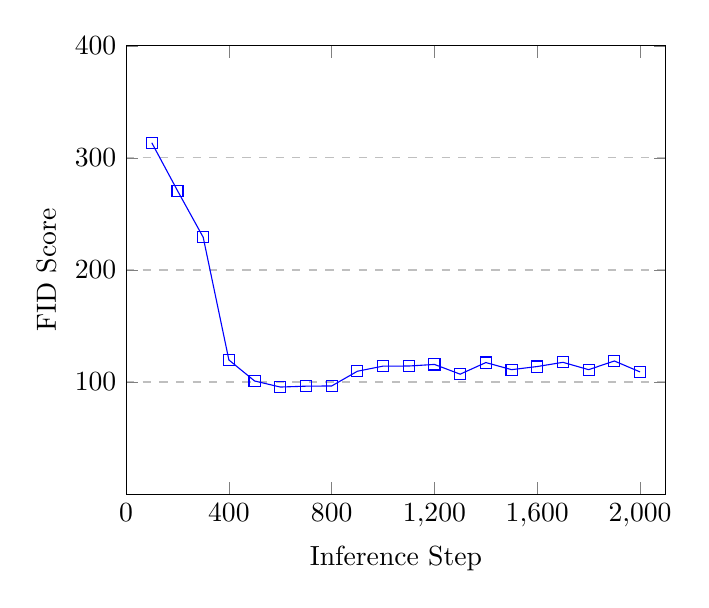
\begin{tikzpicture}
  \begin{axis}[
      xlabel={Inference Step},
      ylabel={FID Score},
      xmin=0, xmax=2100,
      ymin=0, ymax=400,
      xtick={0,400,800,1200,1600,2000},
      ytick={100,200,300,400},
      ymajorgrids=true,
      grid style=dashed,
  ]
  
  \addplot[
      color=blue,
      mark=square,
      ]
      coordinates {
        (100,313.47)(200,270.74)(300,229.2)(400,119.72)(500,100.96)(600,95.55)(700,96.32)(800,96.5)(900,109.64)(1000,114.22)(1100,114.29)(1200,115.73)(1300,107.03)(1400,117.4)(1500,111.05)(1600,113.85)(1700,117.6)(1800,111.06)(1900,118.8)(2000,109.04)
      };
      
  \end{axis}
  \end{tikzpicture}
    \caption{For the Anime Face dataset, as the number of noise additions increased, there was a change in the FID score of the images generated by the diffusion model.}
    \label{fig:anime_face_fid}
  \end{figure}